\documentclass[11pt, oneside]{article}   	% use "amsart" instead of "article" for AMSLaTeX format
\usepackage{geometry}                		% See geometry.pdf to learn the layout options. There are lots.
\geometry{letterpaper}                   		% ... or a4paper or a5paper or ... 
%\geometry{landscape}                		% Activate for for rotated page geometry
\usepackage[parfill]{parskip}    		% Activate to begin paragraphs with an empty line rather than an indent
\usepackage{graphicx}				% Use pdf, png, jpg, or eps§ with pdflatex; use eps in DVI mode
\usepackage{enumitem}
					% TeX will automatically convert eps --> pdf in pdflatex		
\usepackage{amssymb}
\usepackage{float}
\title{Masters' Project \\Michaelmas Progress Report}
\author{Patrick Lewis \\Queens' College}
\date{December 2015}							% Activate to display a given date or no date

\begin{document}
\maketitle
\begin{figure}[H]
    \centering
    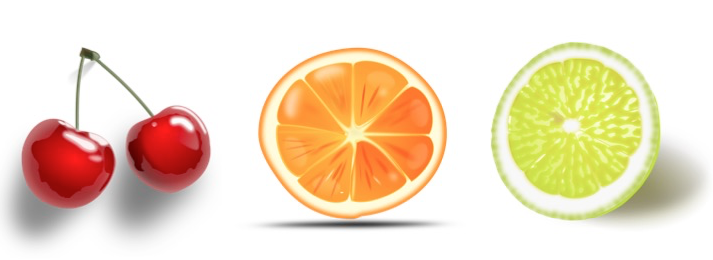
\includegraphics[scale=0.5]{TITLE.png}
\end{figure}
\section{Introduction}
\subsection{Modern Scientific Publishing}
With the widespread adoption of the internet in the late 1990's and 2000's, there were fundamental sweeping changes in the academic publishing landscape. The information revolution allowed publisher's costs to fall dramatically, and there was a mood shift in the academic sphere away from subscription based models, towards giving open and free access to some or all of journal article contents.

Simultaneously, University Department websites began to post records of their recent publications for adverting and informational purposes, usually with hyperlinks to where the article could be fully accessed.

Publishers still protect journal article content and metadata, in some cases, aggressively, in order to look after their intellectual property. The data they hold on article publishing is immensively valuable, and as such, publishers are not willing to give access to their massive metadata holdings. There is a well known saying in Data Science from Tim O'Reilly, ``The Guy with The Most Data Wins" \cite{HEWHOHASDATA}. As such, it is unlikely that academic publishing companies will release their data for analysis by the public.
\subsection{Motivation}
The publishing data, when collected and analysed using machine learning and big data techniques, can yield valuable insights into the direction of shifting academic focus, where world leading research is being carried out, and offers the possibility of procedural categorisation of research. The possibilities do not end there, and large datasets are almost infinitely mine-able for interesting insights. For an academic institution like the University of Cambridge, there are two main motivations for mining the data of the publishing landscape:
\begin{itemize}
\item{Purely Academic insights such as examination of the landscape's features , finding structural information and concealed relationships, in order to better understand how scientific information is spread throughout the world}
\item{Actionable insights, such as identifying where effective collaborations could be set up, prediction of where funding may been allocated, and identification of future areas of academic interests so that internal resources can be intelligently applied}
\end{itemize}
\subsection{Aims}
There are two main aims for the project, broken down below.
\begin{itemize}
\item{Data Collection - A scalable, legal and useful programmatic approach to scrape the online publishing landscape to collect as much useful data as possible.}
\item{Data Analysis - Once the data has been collected, Machine learning and statistical techniques should be applied to try and find insights within the data.}
\end{itemize}
The data analysis for such a large, rich dataset is a potentially never ending process. The strategy adopted is to focus on answering a smaller simpler research question first, building a structure to robustly test and answer that hypothesis and then to move on to new research questions.
As such, the first research question will be to build a system that can analyse the similarity between scientific authors. This will enable us to find where some authors are publishing qualitatively similar work and to investigate the possibility of them collaborating. 
The framework upon which this research question is used immediately suggests new, similar questions that can be answered. As such, it will be a primary aim of the project to expose a useful framework for future probing to be facilitated.

From a technical point of view, the aims of the project are as follows:
\begin{itemize}
\item{Provide documented, maintainable code}
\item{Provide a system that is as automated as possible}
\item{Provide a system that will automatically evolve and improve as time goes on}
\item{Provide a system that will not entropically lose data or suffer data degradation}
\item{Provide a system that produces interpretable, useful outputs}
\end{itemize}
The focus is on ensuring that the result of the project is a system that will continue to be useful after the programmer has left. This will require decent documentation discipline, and systems in place to manage crashing.
\section{First Steps}
\subsection{Generating Xpaths}
The initial focus was on developing a strategy to scrape records off an unseen webpage.
Webpages are written in a tree-like structure using a markup language called HTML, (HyperText Markup Language). A very basic webpage is shown in Figure~\ref{fig:HTMLTREE}
\begin{figure}
    \centering
    \textbf{HTML and XPaths}\par\medskip
    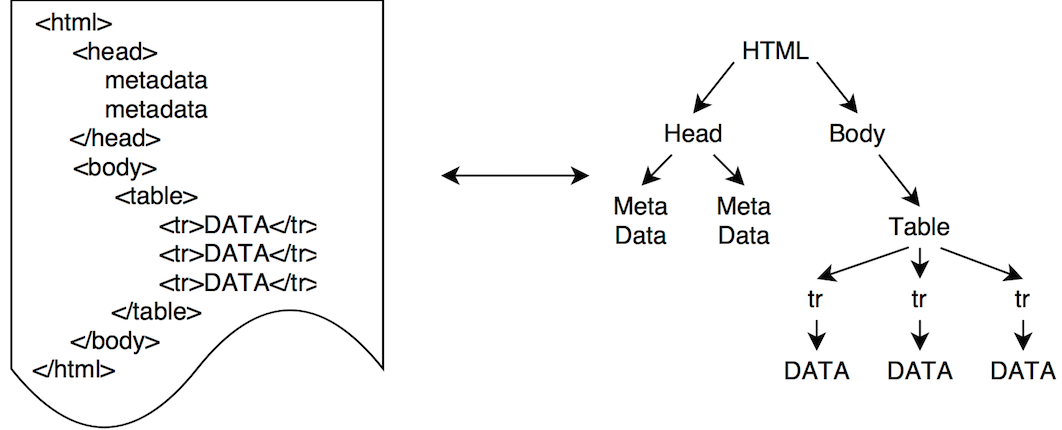
\includegraphics[scale=0.3]{HTMLTREE2.png}
    \caption{Tree representation of HTML code\label{fig:HTMLTREE}}
\end{figure}

When a webpage is accessed, the html code is sent over the internet to the user, and the browser e.g. Firefox, interprets it and displays the webpage in a human readable format. When scraping a page for information, the html code itself is scraped. The programmer must  write a program that accesses the useful parts of the webpage and stores the required information. In the above simplified example, it is shown that the html code represents a tree structure, and the useful data is at the bottom of the 'body' branch. In order to store the DATA fields, the programmer must provide what is known as the XPath to that node in the tree. The Xpath is just a direction to the data, and in the example above, the DATA fields are accessed via XPath:\begin{center} \texttt{//HTML/Body/Table/Tr/*}\end{center}
The Xpath is a required part of any scraping strategy. The first problem with scraping potentially millions of webpages, is how the Xpath (potentially very complicated, and certainly different for every single website) can be generated. The initial approach was to write a tree analysis suite that would give the xpath of the most 'probable' data entries. This worked by finding the most repeated substructure within the entire tree, and by using heuristics, parameters could be adjusted to automatically generate the xpath to the useful data with decent efficiency. 
The core of the algorithm is shown below: 
\begin{sloppypar}
\begin{enumerate}
\item \texttt{Start at trunk of tree}
\item \texttt{Count the number of descendants of each child of the current node}
\item 
\begin{enumerate}
\item \texttt{Check if all child notes are all within a threshold of similarity to each other}
\item \texttt{Check there are more than a required threshold number of child nodes}
\item \texttt{Check the average similarity between child nodes is above a certain threshold}
\item \texttt{Check that the proportion of child nodes that are considered `similar' is above a certain threshold}
\end{enumerate}
\item \texttt{If all of (a)-(d) are true, this node contains the required data and the XPath has been found. Otherwise, move down to the child node with the greatest number of descendants and return to step 2}
\end{enumerate}
\end{sloppypar}
The thresholds mentioned in steps 3.(a)-(d) are adjustable parameters set at reasonable values. This approach was successful for webpages with very large numbers of records on them, as the algorithm searches for the largest, most frequently repeating structural unit in the tree. If there are not vast numbers of records on the page, the method can fail.
As such, it is not flexible enough a strategy, and whilst useful and still the quickest automated way to generate Xpaths for webpages with many hundreds of records on them. A different strategy has been been adopted, please see section~\ref{sec:COLLECTIONSTRATEGY}.
\subsection{CAMSIM and BATHSIM Mini Projects}
A significant part of the first few weeks of the project were dedicated to selecting and learning the appropriate technologies to achieve the goal. The CAMSIM and BATHSIM projects were small proof of concept projects to explore how the different technologies work together, and to prototype a system architecture.
The techologies used are:
\begin{enumerate}
\item Python 2.7.10 programming language. A modern and flexible interpreted programming language widely adopted by the scientific community, python 2 has many useful libraries available, optimised for use.
\item MongDB database - MongoDB is becoming one of the most popular databases for data intentsive applications [CITATION NEEDED]. MongDB is a schema-less noSQL database - it records objects as individual, unstructured elements rather than in tables. This is well suited to the task as complete data is not always available during large scraping operations. There are also well supported python drivers for MongoDB. 
\item Anaconda Environment - Anaconda is a python distribution/virtual environment, allowing quick use of external python packages, and fast generation of distributions to deploy on new machines.
\item Scrapy Scraping suite - A well supported end to end scraping framework for python, allowing fast, scalable web scraping. 
\item Gensim - A Natural Language Processing and Machine Learning suite for Python. Their libraries are C optimised and widely used and verified.
\end{enumerate}

\begin{figure}
    \centering
    \textbf{CAMSIM and BATHSIM Architecture}\par\medskip
    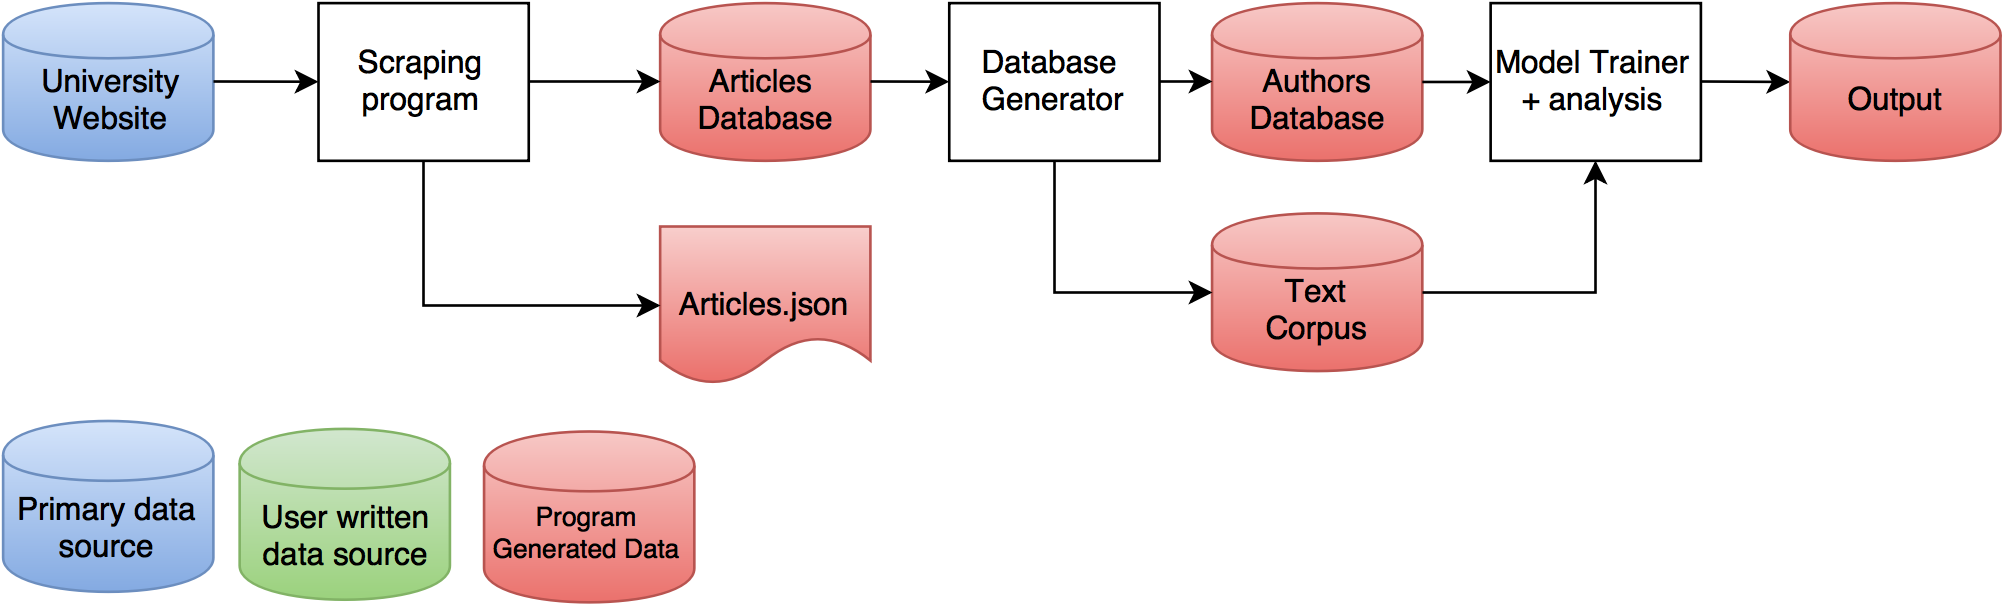
\includegraphics[scale=0.23]{CAMSIM.png}
    \caption{Flow Chart Diagam representing CAMSIM and BATHSIM structure \label{fig:CAMSIM}}
\end{figure}

BATHSIM and CAMSIM projects use all of the above technologies with an architecture shown in Figure ~\ref{fig:CAMSIM}. The programatic flow is represented above. BATHSIM and CAMSIM have the same structure, and the only difference is the source data for CAMSIM is provided by University of Chemistry Department at \texttt{ http://www.ch.cam.ac.uk/publications} whereas BATHSIM's source is the data provided by the Bath University Chemistry department, at \texttt{http://opus.bath.ac.uk/view/divisions/dept=5Fchem.html}. A custom written scraping program collects the data which is placed into a database and exported as a human readable .JSON text file. A second program then creates databases of individual authors and a corpus of all the titles and collected abstracts. As discussed in the section ~\ref{sec:ANALYSIS}, this corpus is used to train a Word2Vec style model that generates a vector representation of an author's published work. The dot product cosines between authors' vectors are computed and outputted as a measure of their similarity.
\section{Collection Strategy}
The main problem encountered so far is how to scrape large numbers of websites for records without writing individual time consuming scraping scripts and finding Xpaths for every website visited, as was used in CAMSIM and BATHSIM. The possible solution is using `regular expressions' pattern matching techniques on DOIs. DOIs are explained in detail in section \ref{sec:DOI}. The proposed collection strategy, which is 90\% complete, is then described in section \ref{sec:CHERRY}.
\subsection{DOI}
\label{sec:DOI}
DOIs (document object identifiers) are identifier strings used access journal articles. DOIs can issued by a number of accredited issuing bodies, although the vast majority of scientific articles are issued by CrossRef, a not-for-profit body comprised from Publishers International Linking Association (PILA), a loose association of many academic publishers \cite{CROSSREF}. A DOI is usually included in a citation or record, and by pre-pending a DOI string with the url stub ``http://dx.doi.org/", DOI.org will redirect the request to the desired academic journal entry on the publishers website. All articles published by large established publishers will have a DOI registered against them.

DOIs have a somewhat loose structure, and the anatomy of a DOI is shown in figure \ref{fig:DOI}.

\begin{figure}[H]
    \centering
    \textbf{Anatomy of a DOI}\par\medskip
    \includegraphics[scale=0.15]{DOI2.png}
    \caption{Doi structure. The structure consists of a numeric prefix (X and Y must be integers) and alphanumeric suffix (Z can be any UTF-8 encoded Character) \label{fig:DOI}}
\end{figure}
DOIs consist of 2 sections, the prefix and suffix. The Prefix is subdivided into a Directory indicator (always integer `10') separated from a registrant code assigned by the issuing body. REgistrant codes are numeric and can be of any length, however they are almost invariably 4 integers long. Registrant codes can have further subdivisions seperated by full stops. 

\subsection{Cherry Data Collection Program}
\label{sec:CHERRY}

\label{sec:COLLECTIONSTRATEGY}
\section{Analysis}
\label{sec:ANALYSIS}
\subsection{Algorithm}
\subsection{Data processing}
\section{Next Steps}
\section{Bibliography}
\begin{thebibliography}{9}
\bibitem{HEWHOHASDATA} O'Reilly (2012) \emph{Tim O'Reilly interviewed by Forbes Editor Jon Bruner} Available at: https://www.youtube.com/watch?v=wNLhFi3XhIE (accessed 24 November 2015)
\bibitem{CROSSREF}
\emph{The Formation of CrossRef: A Short History} (2009) Available at: http://www.crossref.org/08downloads/CrossRef10Years.pdf
accessed 25 November 2015)

\end{thebibliography}

\end{document}  